\documentclass{article} % For LaTeX2e
\usepackage{iclr2026_conference,times}

\input{math_commands.tex}

\usepackage{hyperref}
\usepackage{url}
\usepackage{graphicx}
\usepackage{booktabs}
\usepackage{amsmath,amssymb}
\usepackage{microtype}
\usepackage{subcaption}
\usepackage{enumitem}

\title{Staged Metric-Gated GRPO for Structurally Reliable Visual Numeric Reasoning}

\author{}

\begin{document}

\maketitle

\begin{abstract}
We study a failure mode that is common in reinforcement-learning fine-tuning of vision-language models for visual numeric reasoning: the policy receives correctness pressure before it reliably emits parseable, well-formed, and non-truncated answers. The codebase we analyze implements a staged metric-gated GRPO pipeline around \texttt{Qwen2.5-VL-7B-Instruct}, with four ingredients: (i) phase-wise curriculum over filtered MathVista subsets, (ii) a strict response contract requiring \texttt{<REASONING>} and \texttt{<SOLUTION>} tags, (iii) a reward controller that raises or preserves structure-oriented rewards when checkpoint metrics indicate structural failure, and (iv) checkpoint-side evaluation with alias-based model selection because later RL checkpoints are not always better. Under the repository's internal evaluation protocol, the best large-split Phase C checkpoint improves exact match from 0.375 in a saved pre-refactor baseline snapshot to 0.75 while maintaining 1.0 parseability and zero truncation on the monitored evaluation subset. The strongest empirical pattern is not a smooth accuracy curve, but a two-stage dynamic: smoke runs first stabilize structure, and only then does a larger Phase C continuation produce the main correctness gain. We position this work as an RL systems-and-method paper: the contribution is not a new GRPO loss, but an adaptive training stack that makes GRPO behavior more legible and more robust for visual numeric QA.
\end{abstract}

\section{Introduction}

Reinforcement-learning fine-tuning for language and vision-language models is often described as an accuracy-improving step layered on top of a capable pretrained model. In practice, that framing can be misleading for structured visual reasoning tasks. Before a policy can benefit from correctness reward, it must first produce outputs that are short enough to finish, tagged in a way the evaluator can parse, and stable enough that checkpoint-to-checkpoint comparisons are meaningful. When those prerequisites are missing, RL updates can chase correctness on malformed or truncated outputs, and apparent progress can become highly non-monotonic.

This paper documents and systematizes one concrete solution implemented in the repository: a staged metric-gated GRPO pipeline for MathVista-style visual numeric reasoning. The pipeline does not treat all samples, all rewards, or all checkpoints equally. Instead, it uses explicit curriculum phases, stage-aware data filtering, rule-based reward floors and increments keyed to checkpoint metrics, and alias-based checkpoint selection. The central idea is simple: maintain pressure on structure until structure is empirically stable, and only then increase pressure on exact correctness.

The resulting system is not a new RL objective in the sense of \citet{deepseekmath2024}, \citet{wu2025sppo}, or \citet{noukhovitch2025async}. Rather, it is a training wrapper around TRL's GRPO implementation that addresses a practically important regime: visual numeric QA on a single-GPU, low-memory setup, where structural failures, sparse rewards, and checkpoint regressions make naive continuation brittle. The contribution is therefore algorithmic and operational at the same time: a staged controller around GRPO, not a replacement for GRPO.

Figure~\ref{fig:pipeline} summarizes the full training loop. A base VLM is prepared with LoRA adapters, trained on a stage-filtered phase mixture, evaluated at every checkpoint, and then fed back into a reward controller that changes the next training segment's reward weights. Figure~\ref{fig:stage-matrix} shows that the curriculum is defined as overlapping filtered views over the same underlying MathVista split rather than as disjoint datasets.

\paragraph{Contributions.}
\begin{enumerate}[leftmargin=1.2em]
\item We present a staged GRPO training stack for visual numeric reasoning that separates structure stabilization from later correctness improvement.
\item We formalize the repository's metric-gated reward controller, which guards parseability, formatting, and completion before escalating correctness weight.
\item We show that checkpoint-side evaluation plus alias-based selection is necessary because RL trajectories are non-monotonic in this setting.
\item We provide a code-grounded empirical analysis demonstrating a transition from structural improvement on smoke runs to correctness gains only after larger-split continuation.
\end{enumerate}

\begin{figure}[t]
\centering
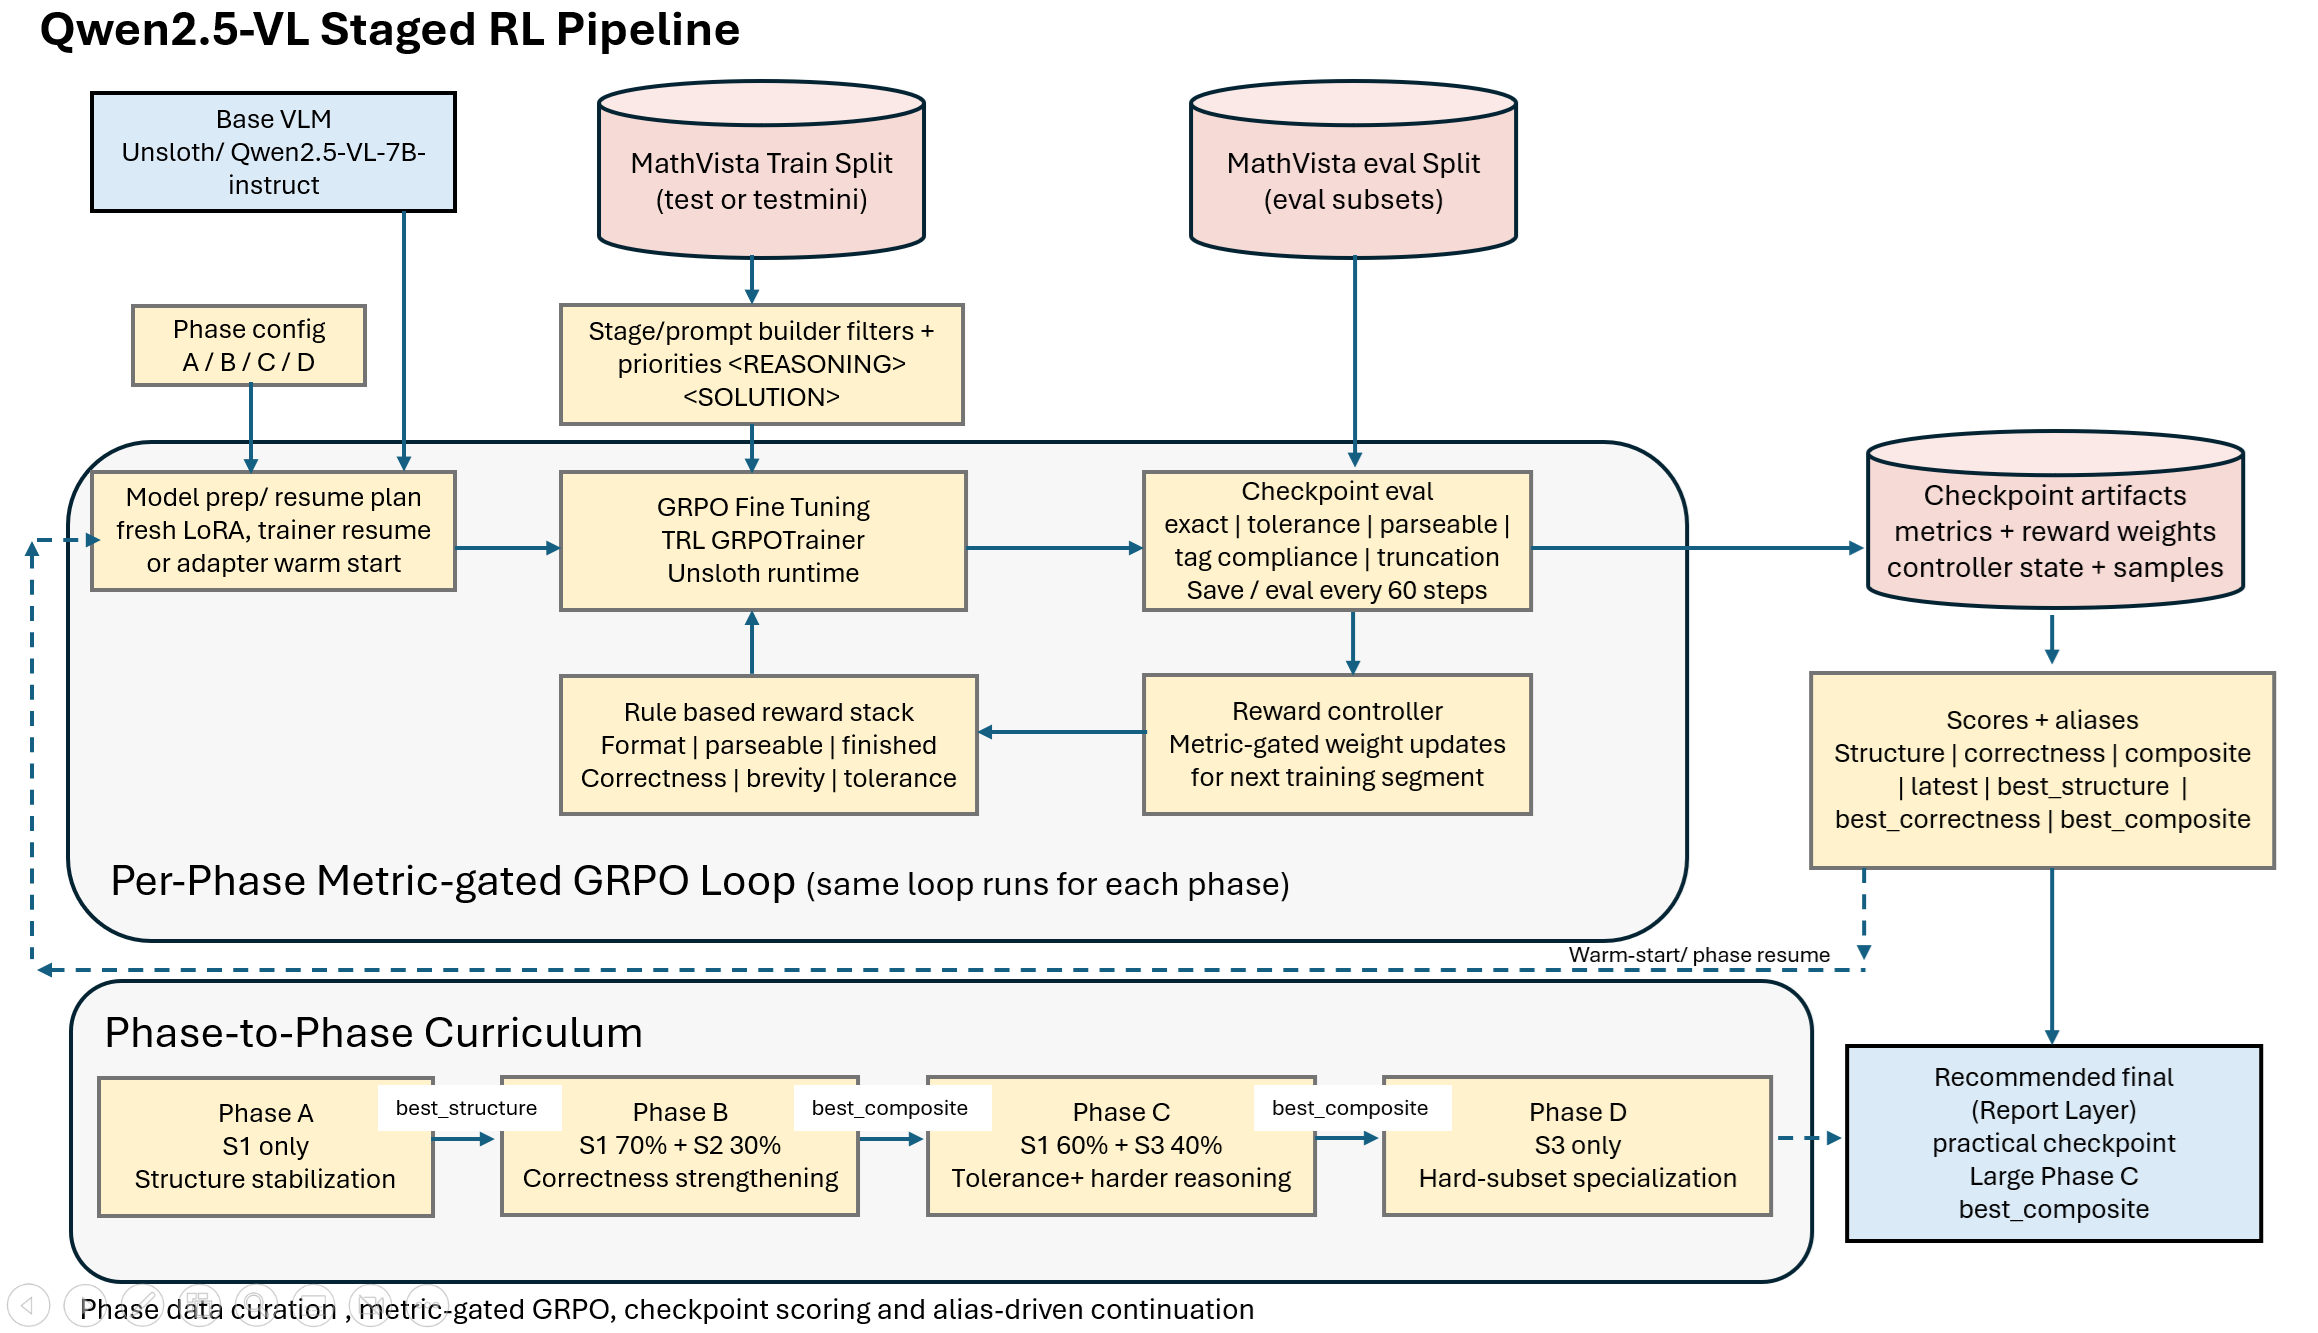
\includegraphics[width=\linewidth]{../../results/plots/staged_training_pipeline_better.png}
\caption{Overview of the repository's staged metric-gated GRPO loop. The pipeline couples phase-specific data curation, GRPO fine-tuning, checkpoint-side evaluation, reward-weight adaptation, and alias-based continuation. Our contribution is the training stack around GRPO rather than a new GRPO loss.}
\label{fig:pipeline}
\end{figure}

\section{Related Work}

\paragraph{RL fine-tuning and preference optimization.}
Recent RLHF and preference-optimization work has focused either on new objectives or on more efficient learning regimes. DeepSeekMath introduced GRPO as a group-relative alternative to PPO for mathematical reasoning \citep{deepseekmath2024}. At ICLR 2025, SPPO proposed a self-play preference objective with a stronger theoretical story than pairwise preference losses \citep{wu2025sppo}, while Asynchronous RLHF studied speed-quality trade-offs in off-policy online RLHF \citep{noukhovitch2025async}. Our paper is orthogonal to these efforts. We do not change the core optimizer. Instead, we study how to wrap GRPO with a curriculum, metric-gated reward scheduling, and checkpoint-selection logic tailored to a failure-prone multimodal setting.

\paragraph{Multimodal mathematical reasoning.}
MathVista exposed the difficulty of mathematical reasoning in visual contexts and remains a useful benchmark for probing diagram, chart, table, and numeric QA behavior \citep{lu2024mathvista}. More recent ICLR papers have attacked the problem from different angles. MAVIS uses a large synthetic data engine plus progressive training for visual mathematics \citep{zhang2025mavis}. CogCoM introduces a chain-of-manipulations mechanism so a VLM can reason through evidential visual steps \citep{qi2025cogcom}. Our contribution is narrower and more operational: we do not build a new dataset or a new manipulation architecture, but show that even with a standard pretrained VLM, RL behavior changes materially when structure, stage difficulty, and checkpoint choice are explicitly controlled.

\paragraph{Curriculum and adaptive reward control.}
The repository is closest in spirit to curriculum and adaptive-control approaches that treat training as a sequence of regimes rather than a single stationary objective. What is distinctive here is the granularity at which adaptation happens: not by epoch, but by checkpoint metrics measured on the current policy. This yields a compact rule set that is easy to audit and directly tied to observable failure modes such as low parseability or high truncation.

\section{Method}

\subsection{Task, response contract, and phase structure}

The code targets MathVista-style visual question answering in which the answer is primarily numeric and free-form. Each prompt is wrapped with a strict output contract:
\begin{quote}
\small\ttfamily
<REASONING> ... </REASONING>\\
<SOLUTION> single numeric answer </SOLUTION>
\end{quote}
This contract matters because the reward functions and the evaluator both depend on extracting a unique solution string from the completion. The pipeline also contains a separate multi-choice scaffold, but that branch is disabled by default and is not part of the core empirical story.

The curriculum is organized into stages and phases. Stages are filtered subsets over the same dataset. In the default configuration:
\begin{itemize}[leftmargin=1.2em]
\item \textbf{Stage 1} restricts to easier English free-form integer questions on synthetic scenes, tables, and natural images.
\item \textbf{Stage 2} broadens to integer and float answers, adding tables, charts, plots, and scientific figures.
\item \textbf{Stage 3} emphasizes harder geometry, scientific-figure, plot, and abstract-scene problems.
\end{itemize}
Phases then mix these stages with different reward emphases:
\begin{itemize}[leftmargin=1.2em]
\item \textbf{Phase A}: Stage 1 only, structure stabilization.
\item \textbf{Phase B}: $0.7$ Stage 1 + $0.3$ Stage 2, correctness strengthening.
\item \textbf{Phase C}: $0.6$ Stage 2 + $0.4$ Stage 3, harder reasoning and tolerance reward.
\item \textbf{Phase D}: Stage 3 only, hard-subset specialization with a longer completion budget.
\end{itemize}

\begin{figure}[t]
\centering
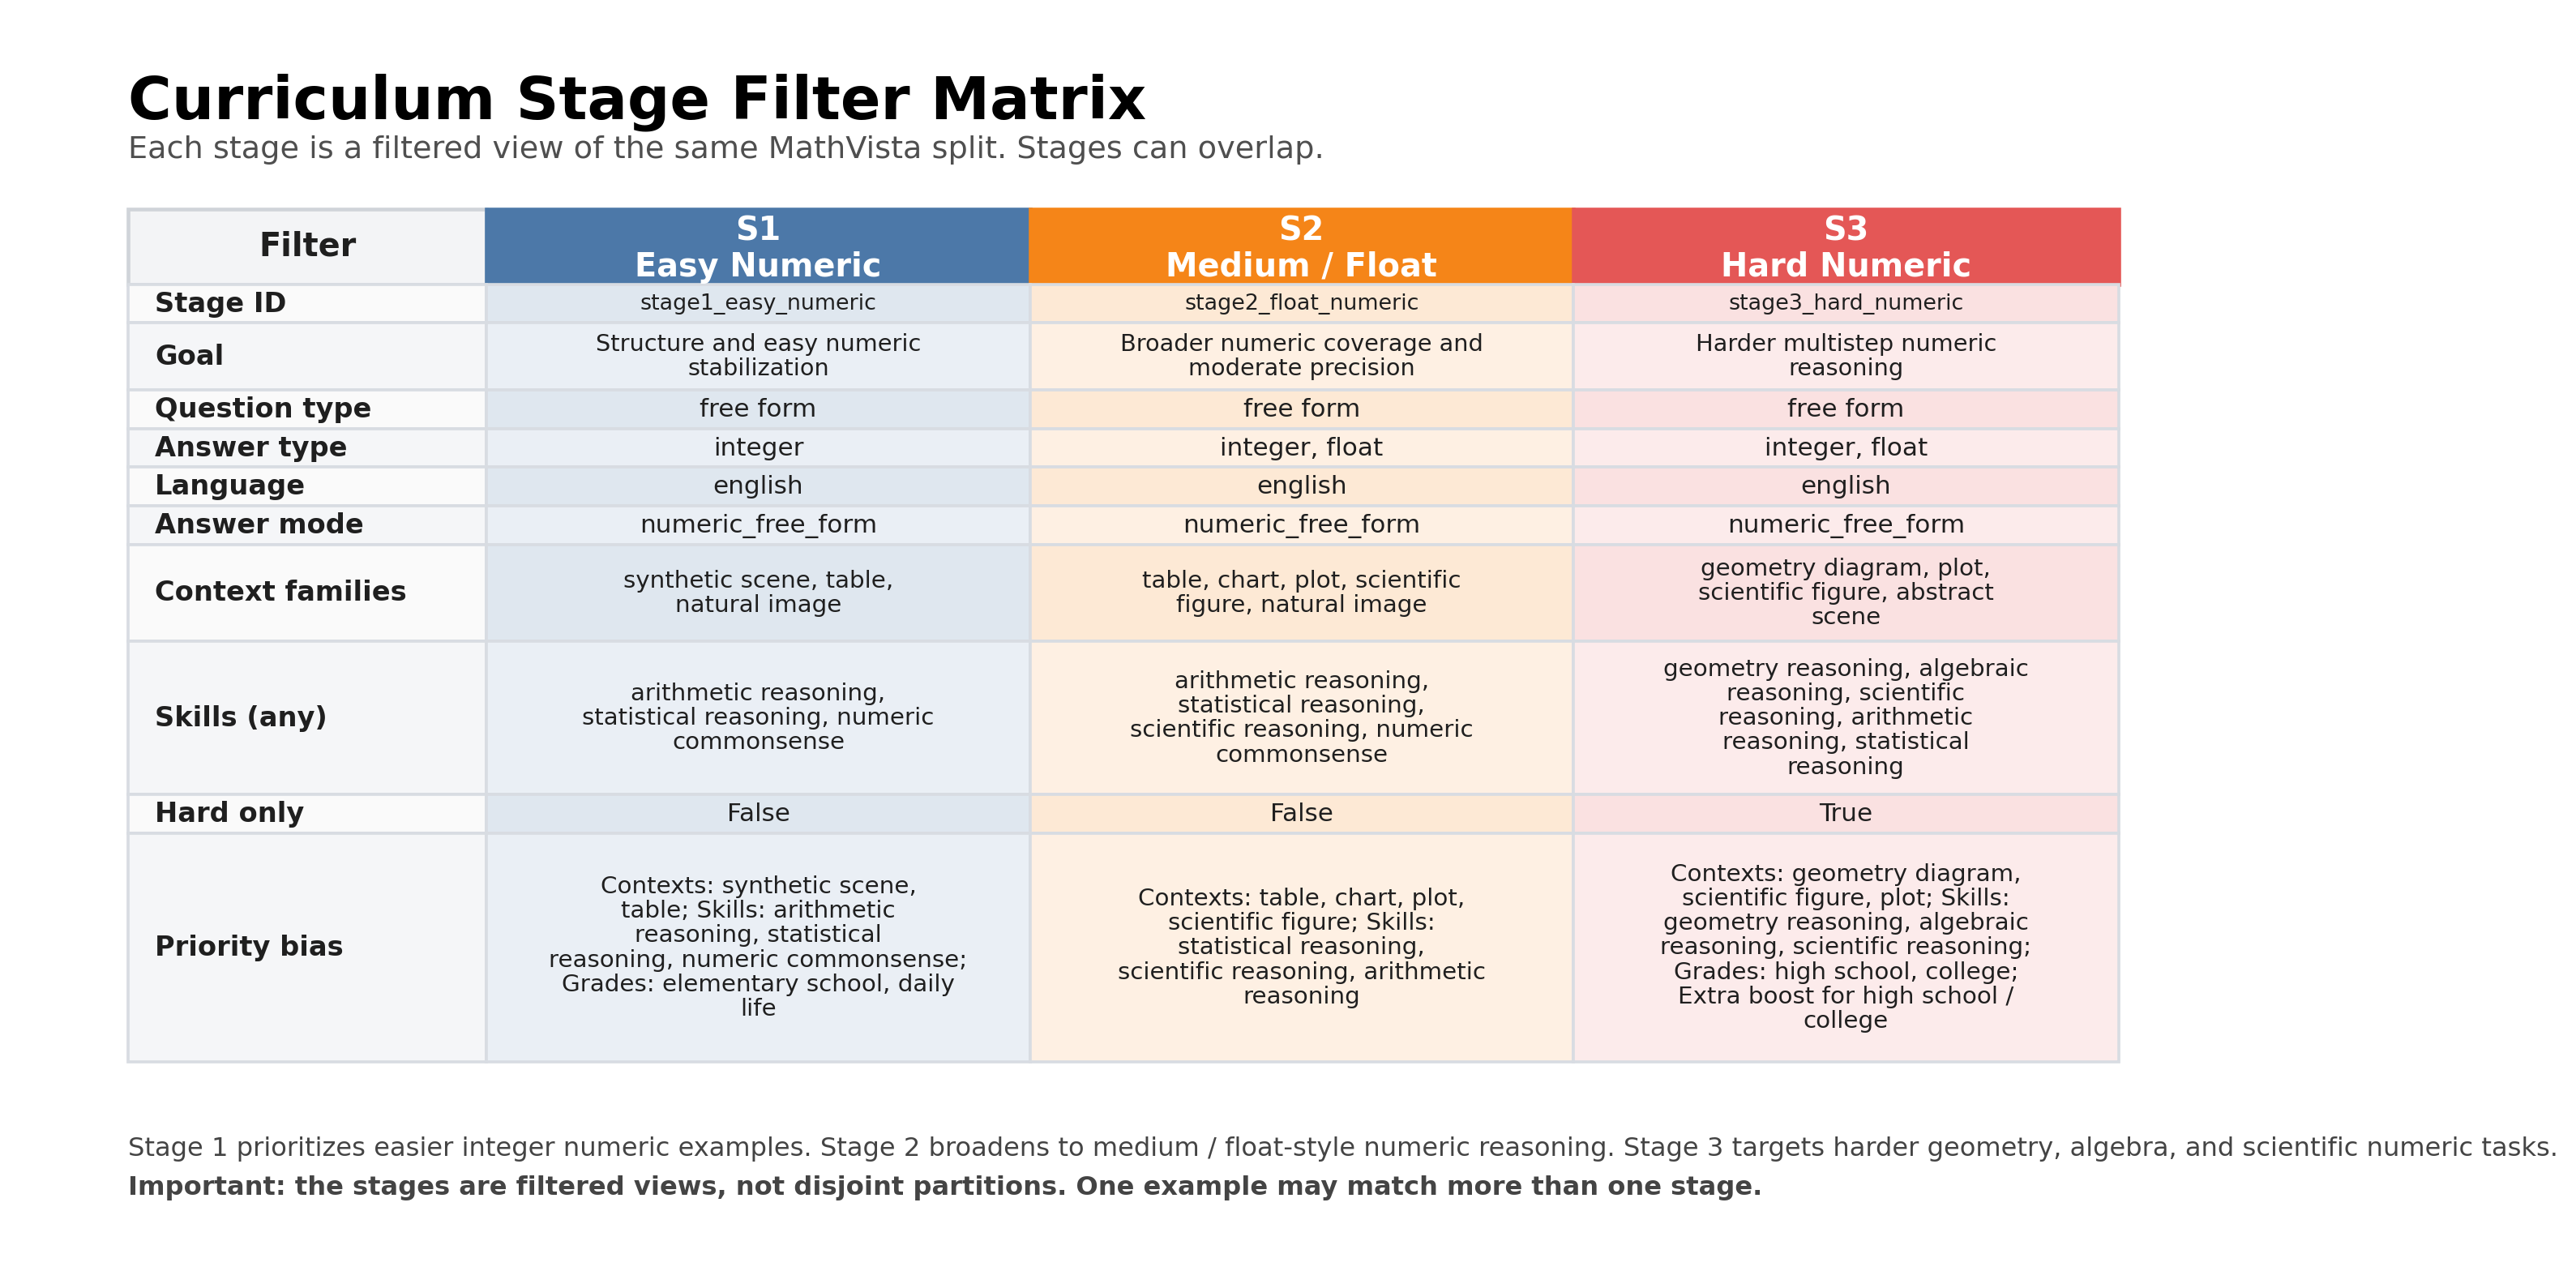
\includegraphics[width=\linewidth]{../../results/plots/stage_filter_matrix.png}
\caption{Filter definitions for the three numeric curriculum stages used in the main training path. The stages overlap and are implemented as filtered views over the same MathVista split, not as fixed disjoint datasets.}
\label{fig:stage-matrix}
\end{figure}

\subsection{Reward decomposition}

For a completion $c$, the repository computes six per-sample reward components:
\begin{equation}
R(c)=\sum_{j=1}^{6} w_j r_j(c),
\end{equation}
where the components correspond to \texttt{format}, \texttt{parseable}, \texttt{finished}, \texttt{correctness}, \texttt{brevity}, and \texttt{tolerance}. The initial weights are phase-specific. For example, Phase A starts with correctness weight $2.0$ but also elevated structure-oriented weights $(1.0,1.0,1.5)$ on format, parseability, and completion; Phase C increases correctness to $5.0$ and activates tolerance reward with weight $1.0$.

Crucially, the implementation never allows structure rewards to decay fully to zero. This is not cosmetic. It encodes the paper's main hypothesis: even when exact match becomes the primary target, structure remains a necessary condition for receiving meaningful reward.

\subsection{Metric-gated reward control}

The reward controller updates weights after each checkpoint evaluation using explicit rules derived from the observed metrics. Let $p$ denote parseable-answer rate, $s$ solution-tag compliance, $r$ reasoning-tag compliance, $m$ malformed rate, $t$ truncation rate, and $e$ exact match. The repository applies the following guards:
\begin{align}
p < 0.85 &\Rightarrow w_{\text{parseable}} \leftarrow \max(w_{\text{parseable}}, 0.75),\\
(s < 0.90)\ \vee\ (r < 0.88)\ \vee\ (m > 0.10) &\Rightarrow w_{\text{format}} \leftarrow \max(w_{\text{format}}, 0.75),\\
(t > 0.15)\ \vee\ (\bar{\ell} > 0.85L) &\Rightarrow w_{\text{finished}} \leftarrow w_{\text{finished}} + 0.25,
\end{align}
where $\bar{\ell}$ is average completion length and $L$ is the completion budget.

Correctness is escalated only when structure is already stable. Stability requires
\begin{equation}
p \ge 0.92,\quad s \ge 0.95,\quad r \ge 0.93,\quad m \le 0.05,\quad t \le 0.08,
\end{equation}
for a two-checkpoint window. If that condition holds and exact-match improvement over the window is below $0.02$, the controller increases correctness weight by $0.50$. All weights are finally clamped to configured bounds. This rule set is intentionally simple enough to audit directly in saved checkpoint artifacts.

\subsection{Checkpoint-side evaluation and alias-based selection}

Instead of treating the most recent checkpoint as the default continuation point, the repository evaluates every saved checkpoint and computes three aggregate scores:
\begin{align}
S_{\text{struct}} &= 0.35\,p + 0.20\,s + 0.20\,r - 0.15\,m - 0.10\,t, \\
S_{\text{corr}} &= 0.70\,e + 0.20\,a_{\text{tol}} + 0.10\,p, \\
S_{\text{comp}} &= 0.45\,e + 0.15\,a_{\text{tol}} + 0.15\,p + 0.10\,s + 0.05\,r - 0.05\,m - 0.05\,t,
\end{align}
where $a_{\text{tol}}$ is tolerance accuracy. These scores back four aliases: \texttt{latest}, \texttt{best\_structure}, \texttt{best\_correctness}, and \texttt{best\_composite}. Cross-phase continuation typically resumes from \texttt{best\_structure} or \texttt{best\_composite}, while same-phase restarts may use full trainer resume from \texttt{latest}. The distinction matters because the code supports both full trainer-state restoration and LoRA-only warm start.

\section{Experimental Setup}

\paragraph{Dataset and model.}
The implementation targets the Hugging Face release of MathVista\footnote{\url{https://huggingface.co/datasets/AI4Math/MathVista}} and loads \texttt{Qwen2.5-VL-7B-Instruct}\footnote{\url{https://huggingface.co/Qwen/Qwen2.5-VL-7B-Instruct}} as the base VLM. For model context we cite the MathVista benchmark paper \citep{lu2024mathvista} and the Qwen2.5-VL technical report \citep{bai2025qwen25vl}.

\paragraph{Runtime profile.}
The repository's main successful runs use the conservative \texttt{kaggle\_t4} profile: 4-bit loading, LoRA rank $8$, max sequence length $1280$, image size $336$, gradient accumulation $4$, two sampled generations per prompt during RL, max prompt length $320$, and max completion length $64$ (or $96$ in Phase D). The trainer uses TRL's \texttt{GRPOTrainer} with sequence-level importance sampling and \texttt{dr\_grpo} loss.

\paragraph{Evaluation protocol and caveat.}
Every saved checkpoint is evaluated on subset builders derived from the configured evaluation split. In smoke runs the code trains on \texttt{testmini} and also evaluates on \texttt{testmini}; in the larger continuation the code trains on \texttt{test} and evaluates on \texttt{testmini}. The evaluation configuration for the Kaggle profile uses only one sampled completion per prompt and caps each subset at two examples. We therefore do \emph{not} present the numbers below as benchmark-comparable MathVista leaderboard results. They are internal, code-grounded measurements used to analyze the training dynamics of this repository.

\paragraph{Reproducibility.}
The repository saves checkpoint-side artifacts including metrics, subset metrics, reward weights, controller state, controller decision logs, prompt-level records, and sample-level JSONL traces. It also includes 26 unit tests covering configuration, data filtering, parsing, checkpointing, evaluation aggregation, controller behavior, and runtime compatibility.

\begin{table}[t]
\centering
\small
\caption{Milestone checkpoints under the repository's internal evaluation protocol. The main empirical pattern is that structure saturates on smoke runs before exact-match gains appear in the larger Phase C continuation.}
\label{tab:milestones}
\begin{tabular}{lcccccc}
\toprule
Checkpoint & EM & Tol & Parse & Malf. & Trunc. & Comp. \\
\midrule
Pre-refactor baseline & 0.375 & 0.375 & 0.641 & 0.359 & 0.242 & 0.405 \\
Smoke Phase A best & 0.500 & 0.500 & 0.500 & 0.500 & 0.500 & 0.400 \\
Smoke Phase B best & 0.500 & 0.500 & 1.000 & 0.000 & 0.000 & 0.600 \\
Smoke Phase C best & 0.500 & 0.500 & 1.000 & 0.000 & 0.000 & 0.600 \\
Large Phase C best & \textbf{0.750} & \textbf{0.750} & \textbf{1.000} & \textbf{0.000} & \textbf{0.000} & \textbf{0.750} \\
Dedicated Phase D best & \textbf{0.750} & \textbf{0.750} & \textbf{1.000} & \textbf{0.000} & \textbf{0.000} & \textbf{0.750} \\
\bottomrule
\end{tabular}
\end{table}

\section{Results}

\subsection{Structure improves before correctness}

Table~\ref{tab:milestones} shows the clearest empirical pattern in the repository. The saved pre-refactor baseline snapshot reaches only $0.641$ parseability with $0.359$ malformed rate and $0.242$ truncation. Smoke Phase A shortens outputs substantially, but structure is still poor. The decisive structural change arrives in Smoke Phase B: parseability, reasoning-tag compliance, and solution-tag compliance all reach $1.0$, while malformed and truncation drop to zero. Yet exact match remains at $0.5$. The implication is that structure improvement and correctness improvement are not synchronized; the former is a prerequisite for the latter.

\begin{figure}[t]
\centering
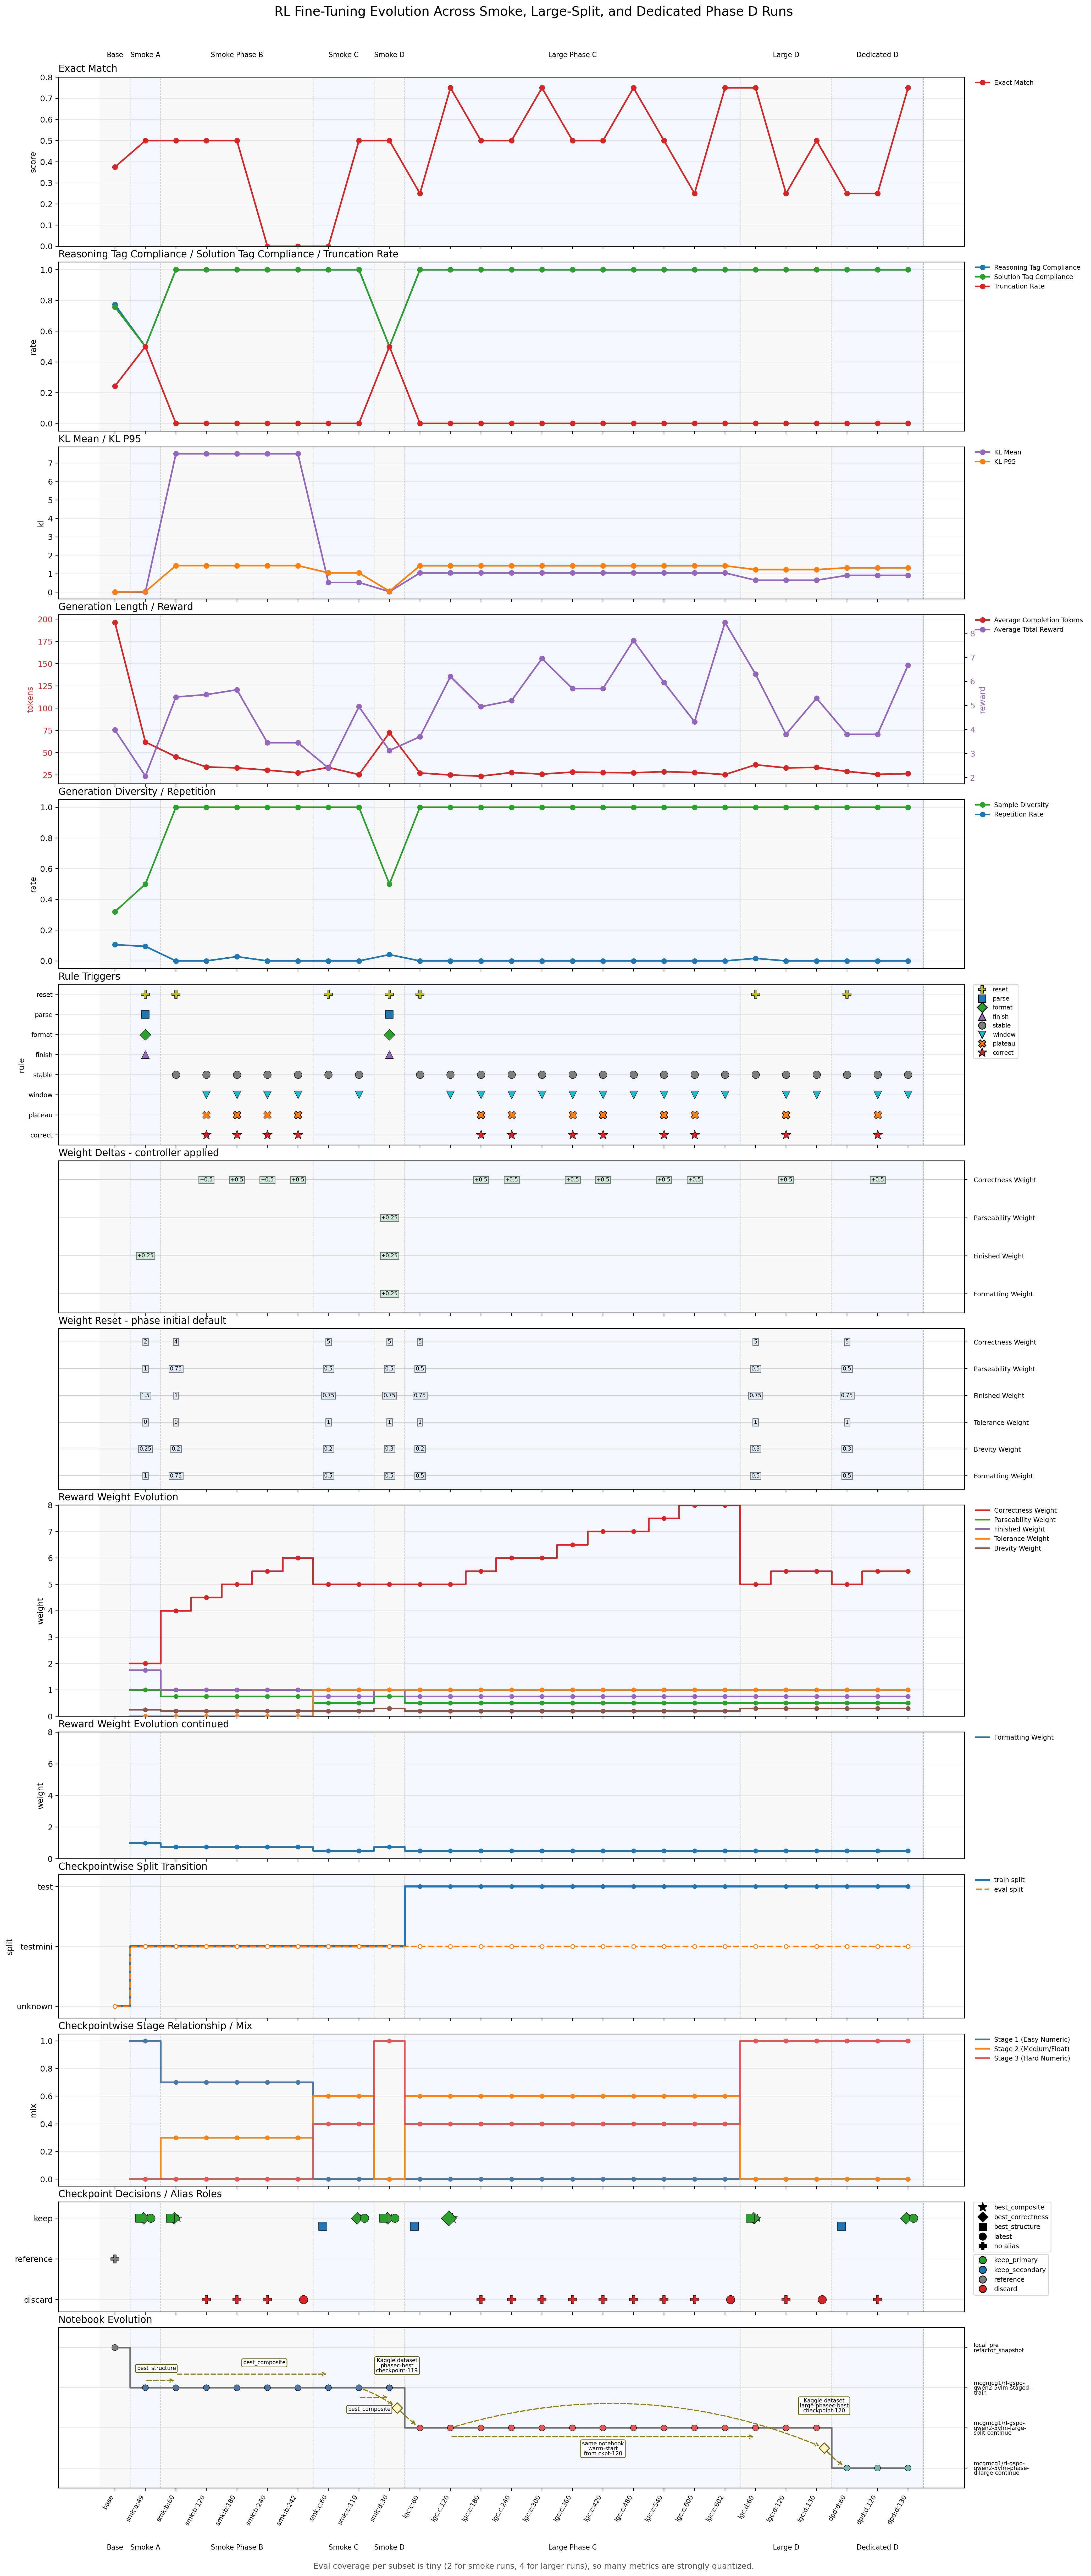
\includegraphics[width=\linewidth,height=0.83\textheight,keepaspectratio]{../../results/plots/evolution_panels_notebook.png}
\caption{Training evolution across milestone checkpoints. The key pattern is a structure-first transition: structural metrics become stable by the smoke Phase B/Phase C regime, while the main exact-match improvement appears only after the larger Phase C continuation.}
\label{fig:evolution}
\end{figure}

Figure~\ref{fig:evolution} makes the transition visually explicit. Once structural metrics saturate, the curves stop telling a ``make outputs valid'' story and start telling a ``make valid outputs correct'' story. This is exactly the regime the controller is designed to create: early checkpoints are allowed to spend reward mass on formatting, parseability, and clean completion; later checkpoints inherit those gains and then receive more correctness pressure.

\subsection{The main gain comes from larger Phase C continuation}

The strongest checkpoint in the repository is the large-split Phase C model at checkpoint 120. Relative to the saved baseline snapshot, exact match rises from $0.375$ to $0.75$, tolerance accuracy from $0.375$ to $0.75$, parseability from $0.641$ to $1.0$, and average completion length shrinks from $196.3$ to $25.0$ tokens. Figure~\ref{fig:base-final} summarizes the before-versus-after comparison.

\begin{figure}[t]
\centering
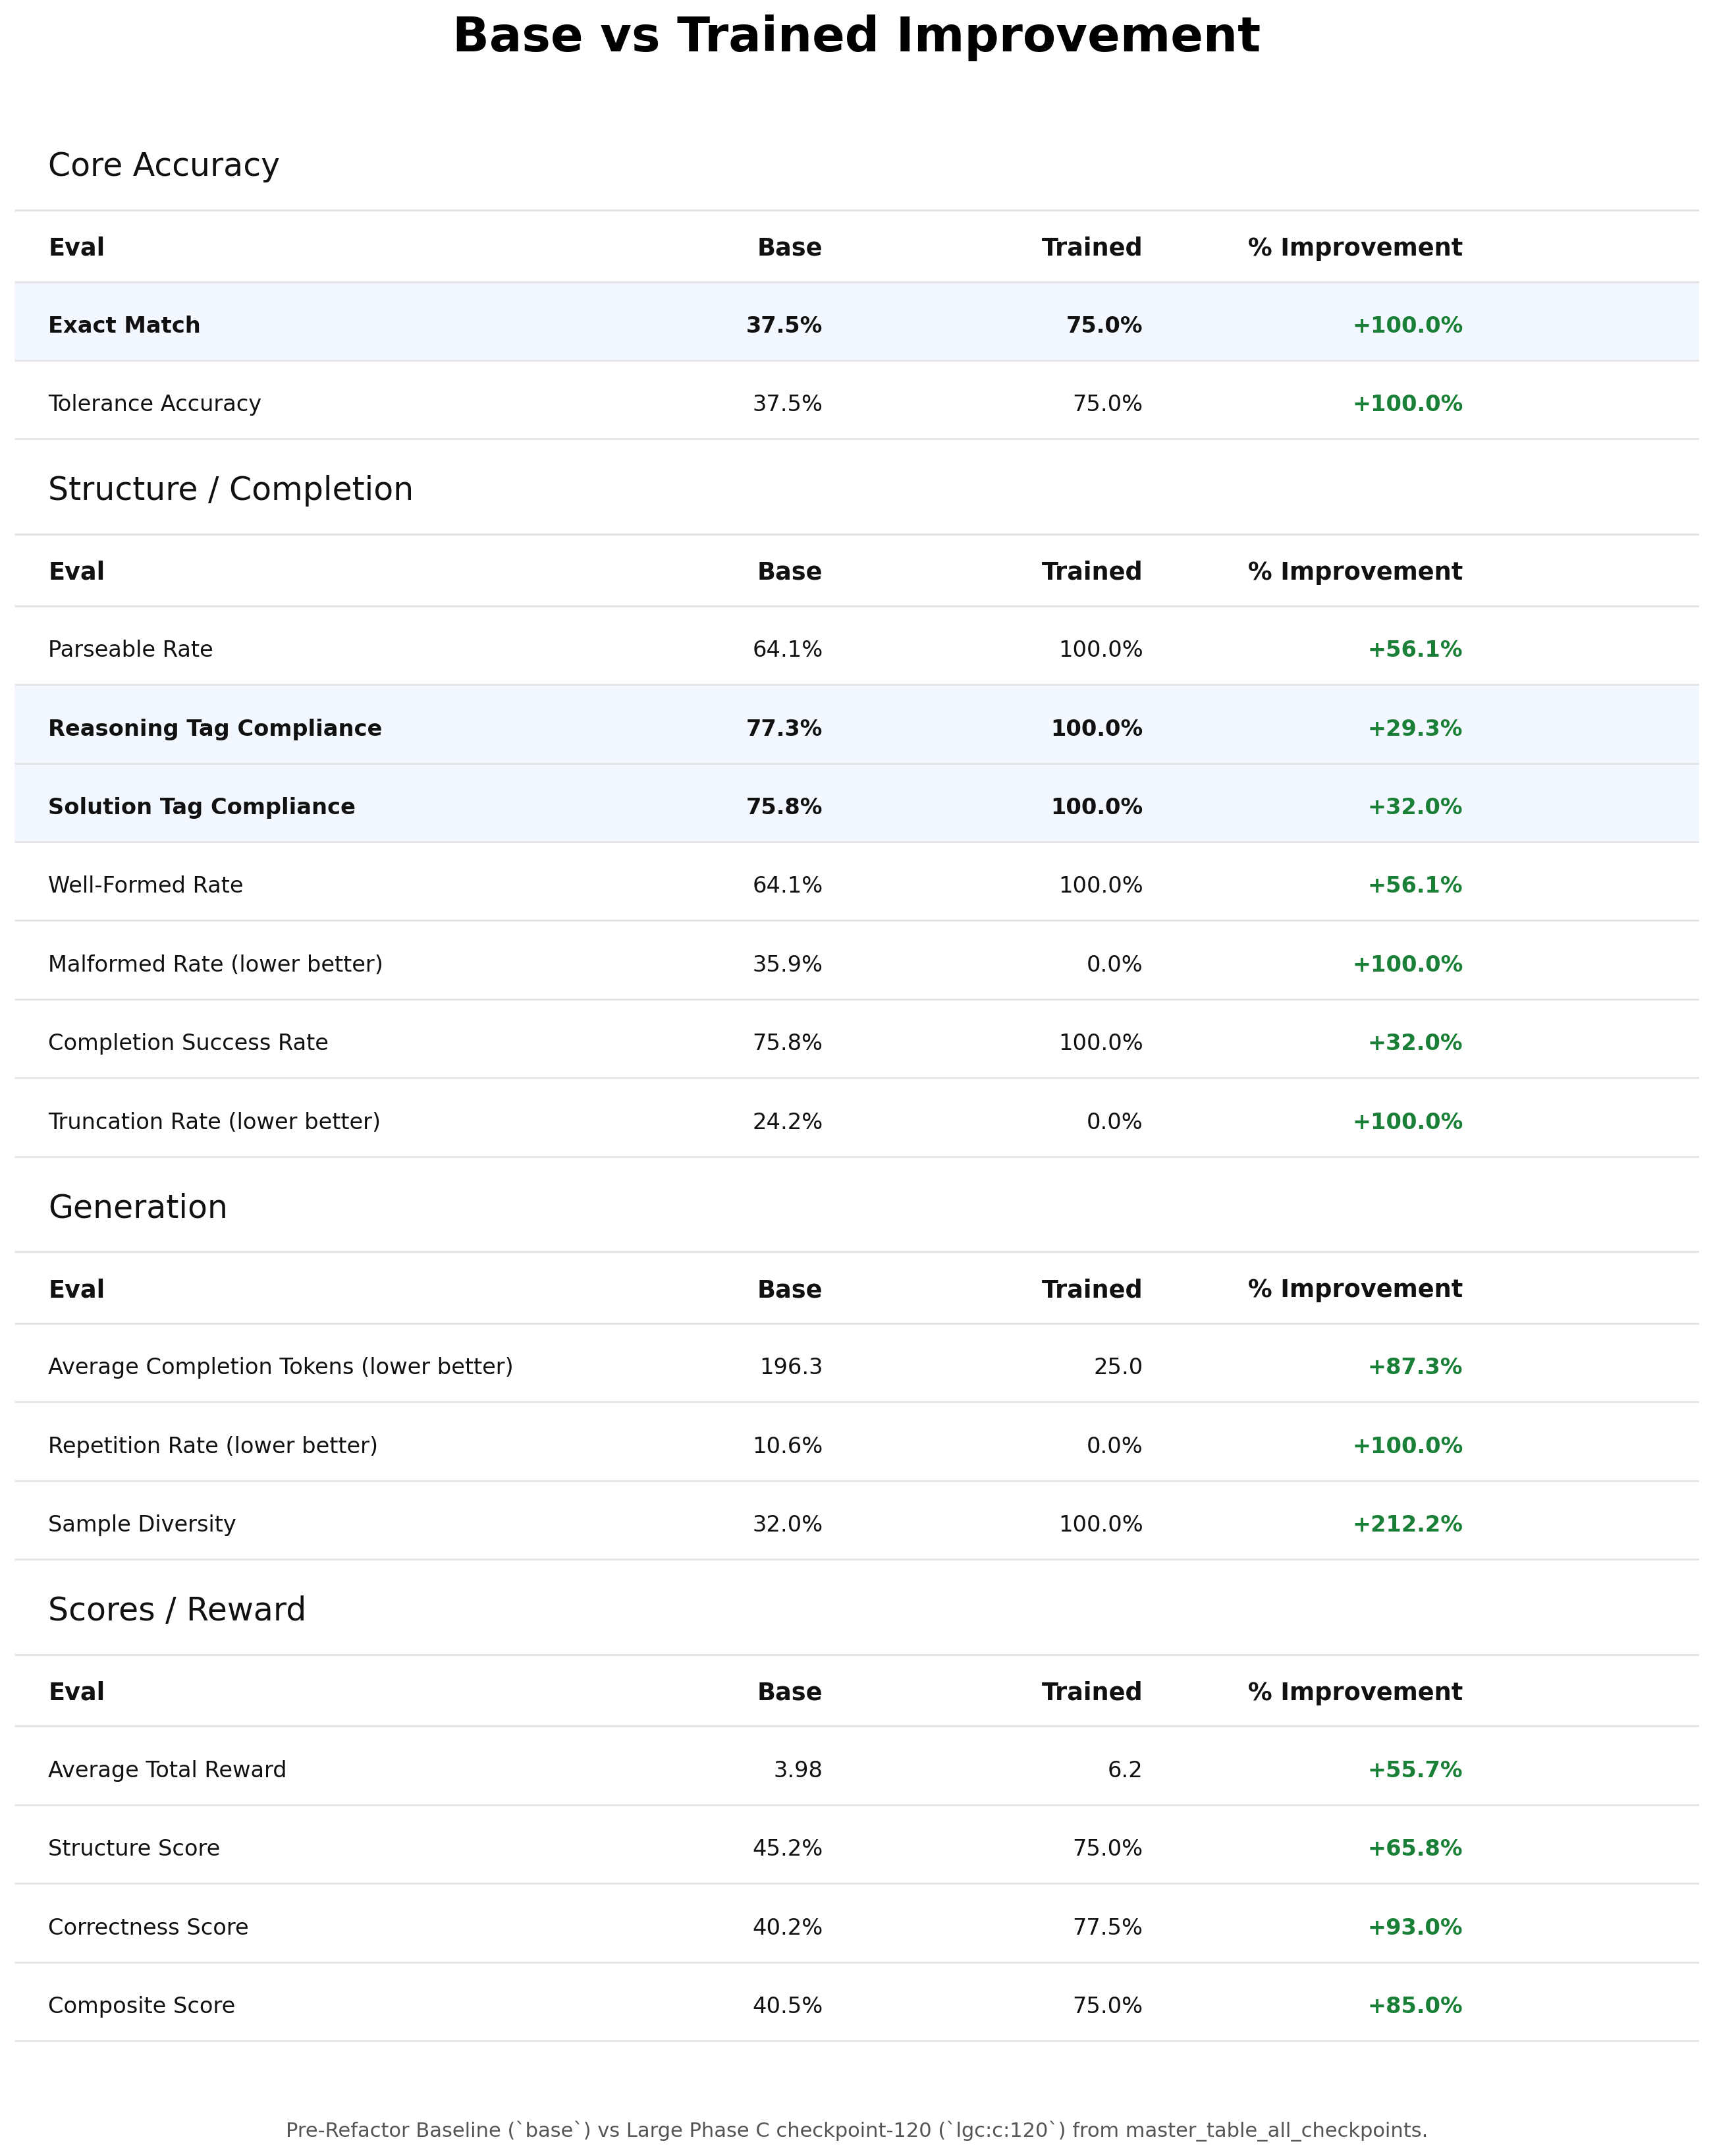
\includegraphics[width=\linewidth,height=0.82\textheight,keepaspectratio]{../../results/plots/base_vs_final_improvement.png}
\caption{Comparison between the saved pre-refactor baseline snapshot and the best large Phase C checkpoint. This figure is most useful as a compact outcome summary; the causal story still comes from the phase-by-phase evolution in Figure~\ref{fig:evolution}.}
\label{fig:base-final}
\end{figure}

An important nuance is that Phase D does not strictly dominate Phase C. A dedicated Phase D run eventually matches the best Phase C score, but it does not exceed it. This matters because it separates two hypotheses: the repository does support hard-subset specialization, but the primary win still comes from the Stage 2/3 mixture in Phase C rather than from Stage-3-only specialization.

\subsection{Checkpoint aliasing is necessary, not cosmetic}

The repository's saved runs provide direct evidence that later checkpoints are not always better. In Smoke Phase B, the best composite checkpoint reaches exact match $0.5$ with perfect structure, while the latest checkpoint regresses to exact match $0.0$ despite keeping parseability and tag compliance at $1.0$. In the large same-notebook Phase D branch, the best checkpoint reaches $0.75$ exact match but the latest checkpoint finishes at $0.5$. This is why alias-based selection is part of the method and not just reporting convenience. Under non-monotonic RL dynamics, resuming from \texttt{latest} can destroy gains that are still present in earlier checkpoints.

\section{Discussion}

The paper's central claim is not that a single rule or single reward fixes multimodal RL. The evidence instead suggests a layered story.

First, a strict response contract makes structural failures measurable. Second, structure-oriented reward components give the optimizer a path to improve those failures before exact match is reliable. Third, a checkpoint-metric controller prevents correctness reward from overwhelming the training signal too early. Fourth, alias-based selection acknowledges that RL trajectories can regress even when the training loop itself is stable.

This combination also clarifies what did \emph{not} happen in the repository. The large gain is not explained by Phase D alone. It is not explained by a monotonic training curve. It is not explained by a larger model, a larger LoRA rank, or a looser generation budget, because the successful large-split runs keep the same low-memory profile. The code-supported causal reading is much narrower: the smoke curriculum stabilizes structure, and the larger Phase C continuation then converts that stable regime into better exact answers.

\section{Limitations and Reproducibility}

The limitations are substantial and should shape how the paper is read.

\begin{itemize}[leftmargin=1.2em]
\item The evaluation subset is tiny in the Kaggle profile, so the reported numbers are useful for internal training analysis but not for broad benchmark claims.
\item The split protocol is repository-specific and, in smoke runs, not held out from training. We therefore avoid comparing directly to published MathVista results.
\item The codebase studies one base model family and one principal hardware profile.
\item The runner is effectively single-GPU even when multiple devices are visible; it does not configure DDP or tensor parallelism automatically.
\item The multi-choice branch (Phase E) and multilingual robustness stage are scaffolded but not part of the core empirical evidence.
\end{itemize}

Despite these limitations, the repository is unusually reproducible for a small RL project. It logs controller decisions at every evaluated checkpoint, persists multiple checkpoint-selection aliases, saves sample-level traces, and includes unit tests for the most failure-prone logic. Those properties make the work especially suitable for an ICLR-style systems-and-method paper whose main contribution is training discipline rather than a new theorem or a new benchmark record.

\section{Conclusion}

We presented a code-grounded study of staged metric-gated GRPO for visual numeric reasoning. The main lesson is simple but practically important: in this setting, structure is not an auxiliary objective that can be ignored once training starts. It is the condition that makes correctness reward usable at all. A phase-wise curriculum, metric-gated reward controller, and alias-based checkpoint selection together turn GRPO from a brittle optimization loop into a more interpretable training process. For this repository, that change is enough to move from a malformed, long-output baseline to a compact and structurally reliable policy whose best large Phase C checkpoint doubles exact match under the internal evaluation setup.

\bibliographystyle{iclr2026_conference}
\bibliography{staged_metric_gated_grpo}

\appendix

\section{Supplementary Figures for Review}

\begin{figure}[t]
\centering
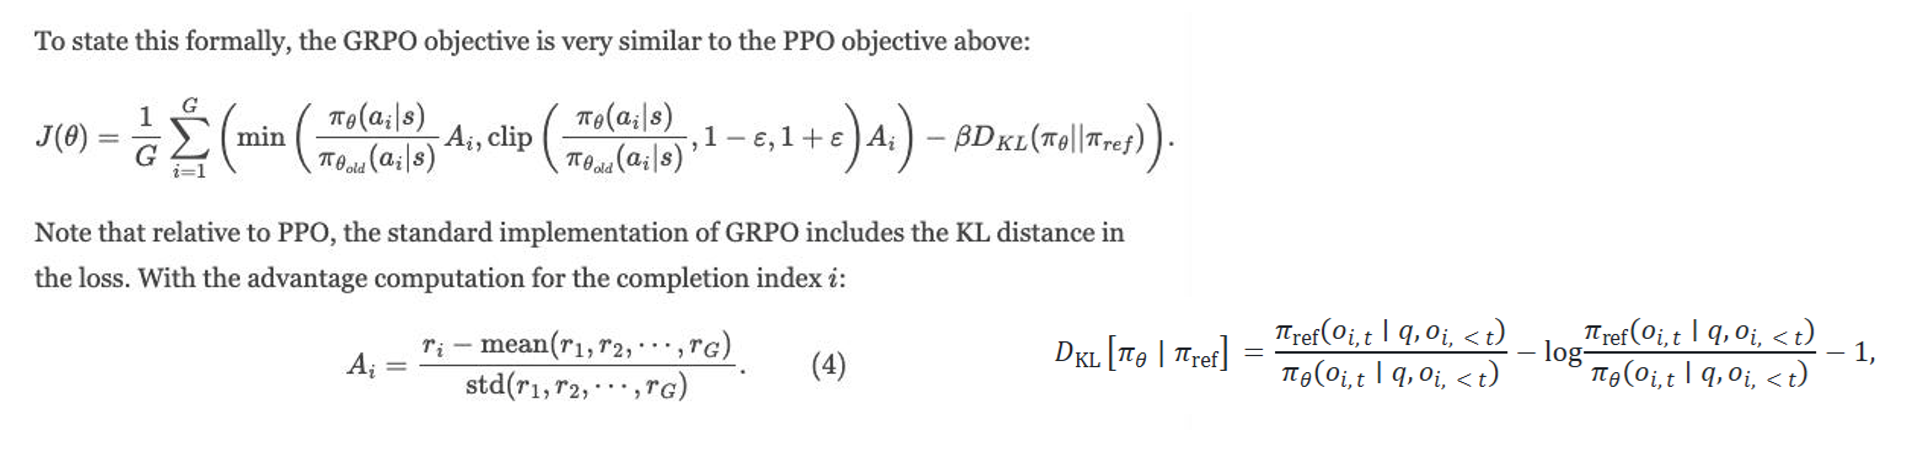
\includegraphics[width=0.92\linewidth]{../../results/plots/GRPO.png}
\caption{Background schematic for GRPO. We include it for intuition only. The contribution of this paper is not a new GRPO loss, but the staged controller and checkpoint-selection stack layered around the existing GRPO trainer.}
\label{fig:grpo-background}
\end{figure}

\begin{figure}[t]
\centering
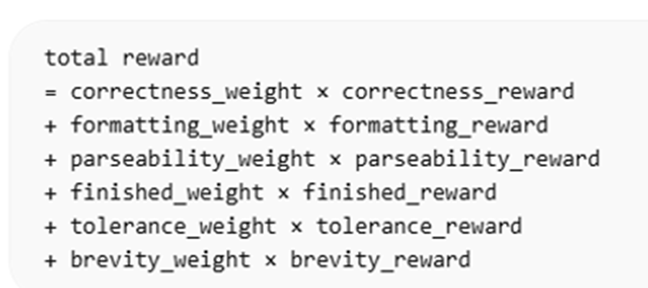
\includegraphics[width=0.65\linewidth]{../../results/plots/Reward_formula.png}
\caption{Compact visual summary of the reward decomposition used in the repository. The exact implementation lives in \texttt{staged\_rl/rewarding.py}; this figure is included as a quick review aid.}
\label{fig:reward-formula}
\end{figure}

\begin{figure}[t]
\centering
\begin{subfigure}[t]{0.49\linewidth}
\centering
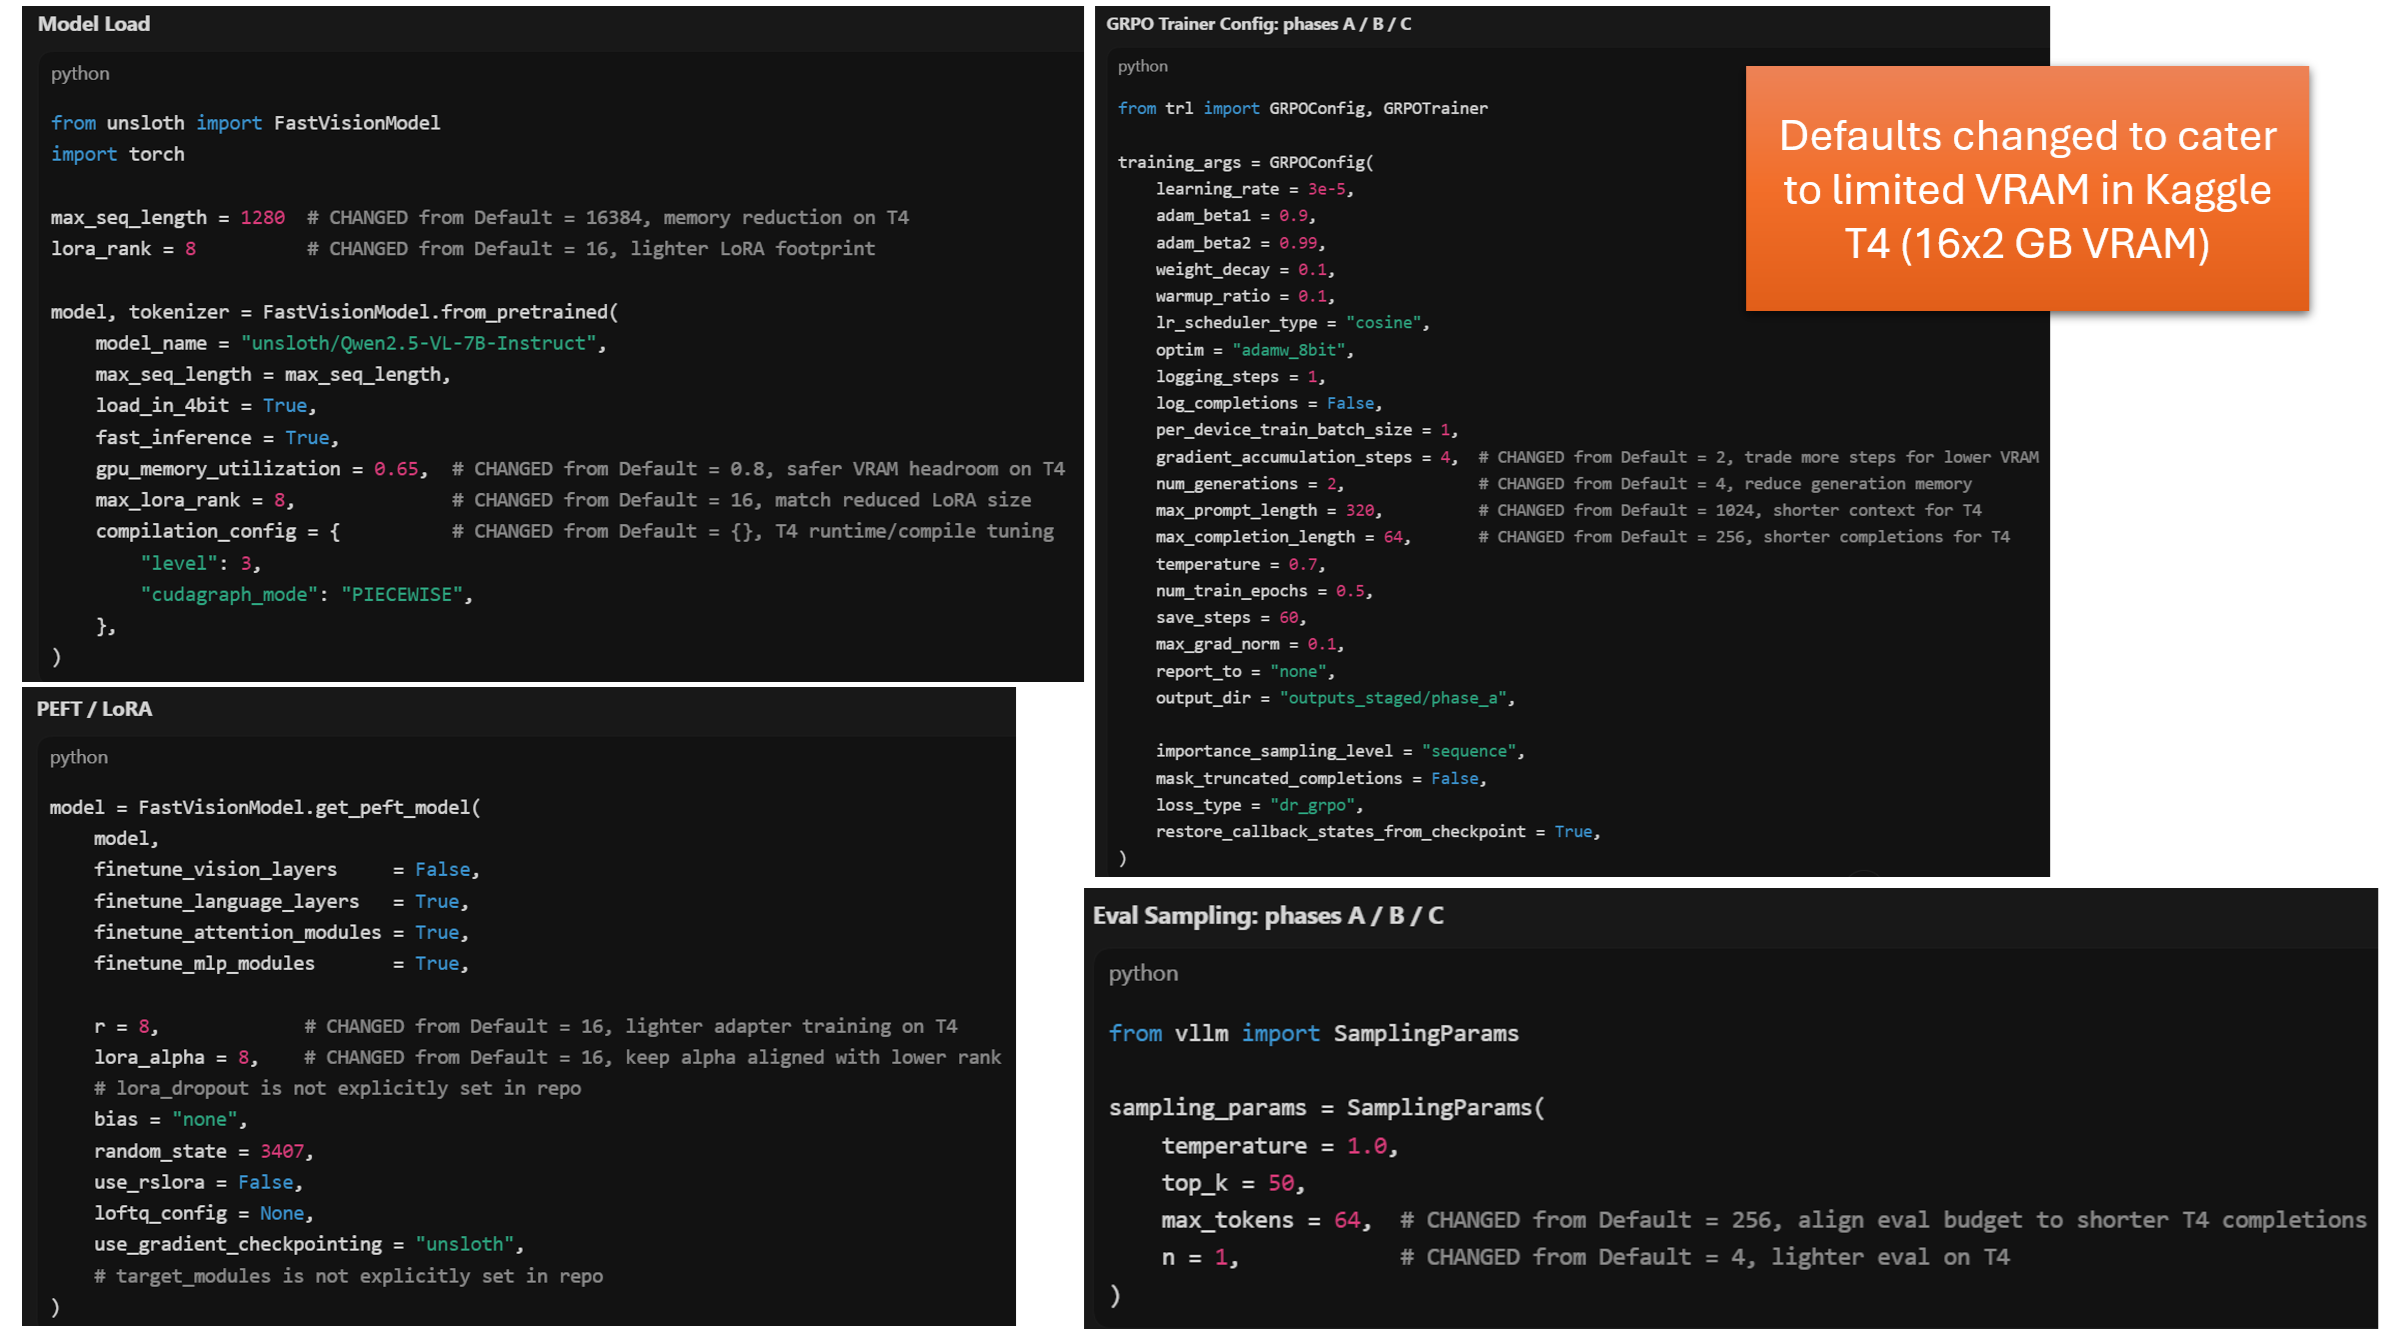
\includegraphics[width=\linewidth]{../../results/plots/Parameter_changes.png}
\caption{Primary hardware-profile and runtime changes.}
\end{subfigure}
\hfill
\begin{subfigure}[t]{0.49\linewidth}
\centering
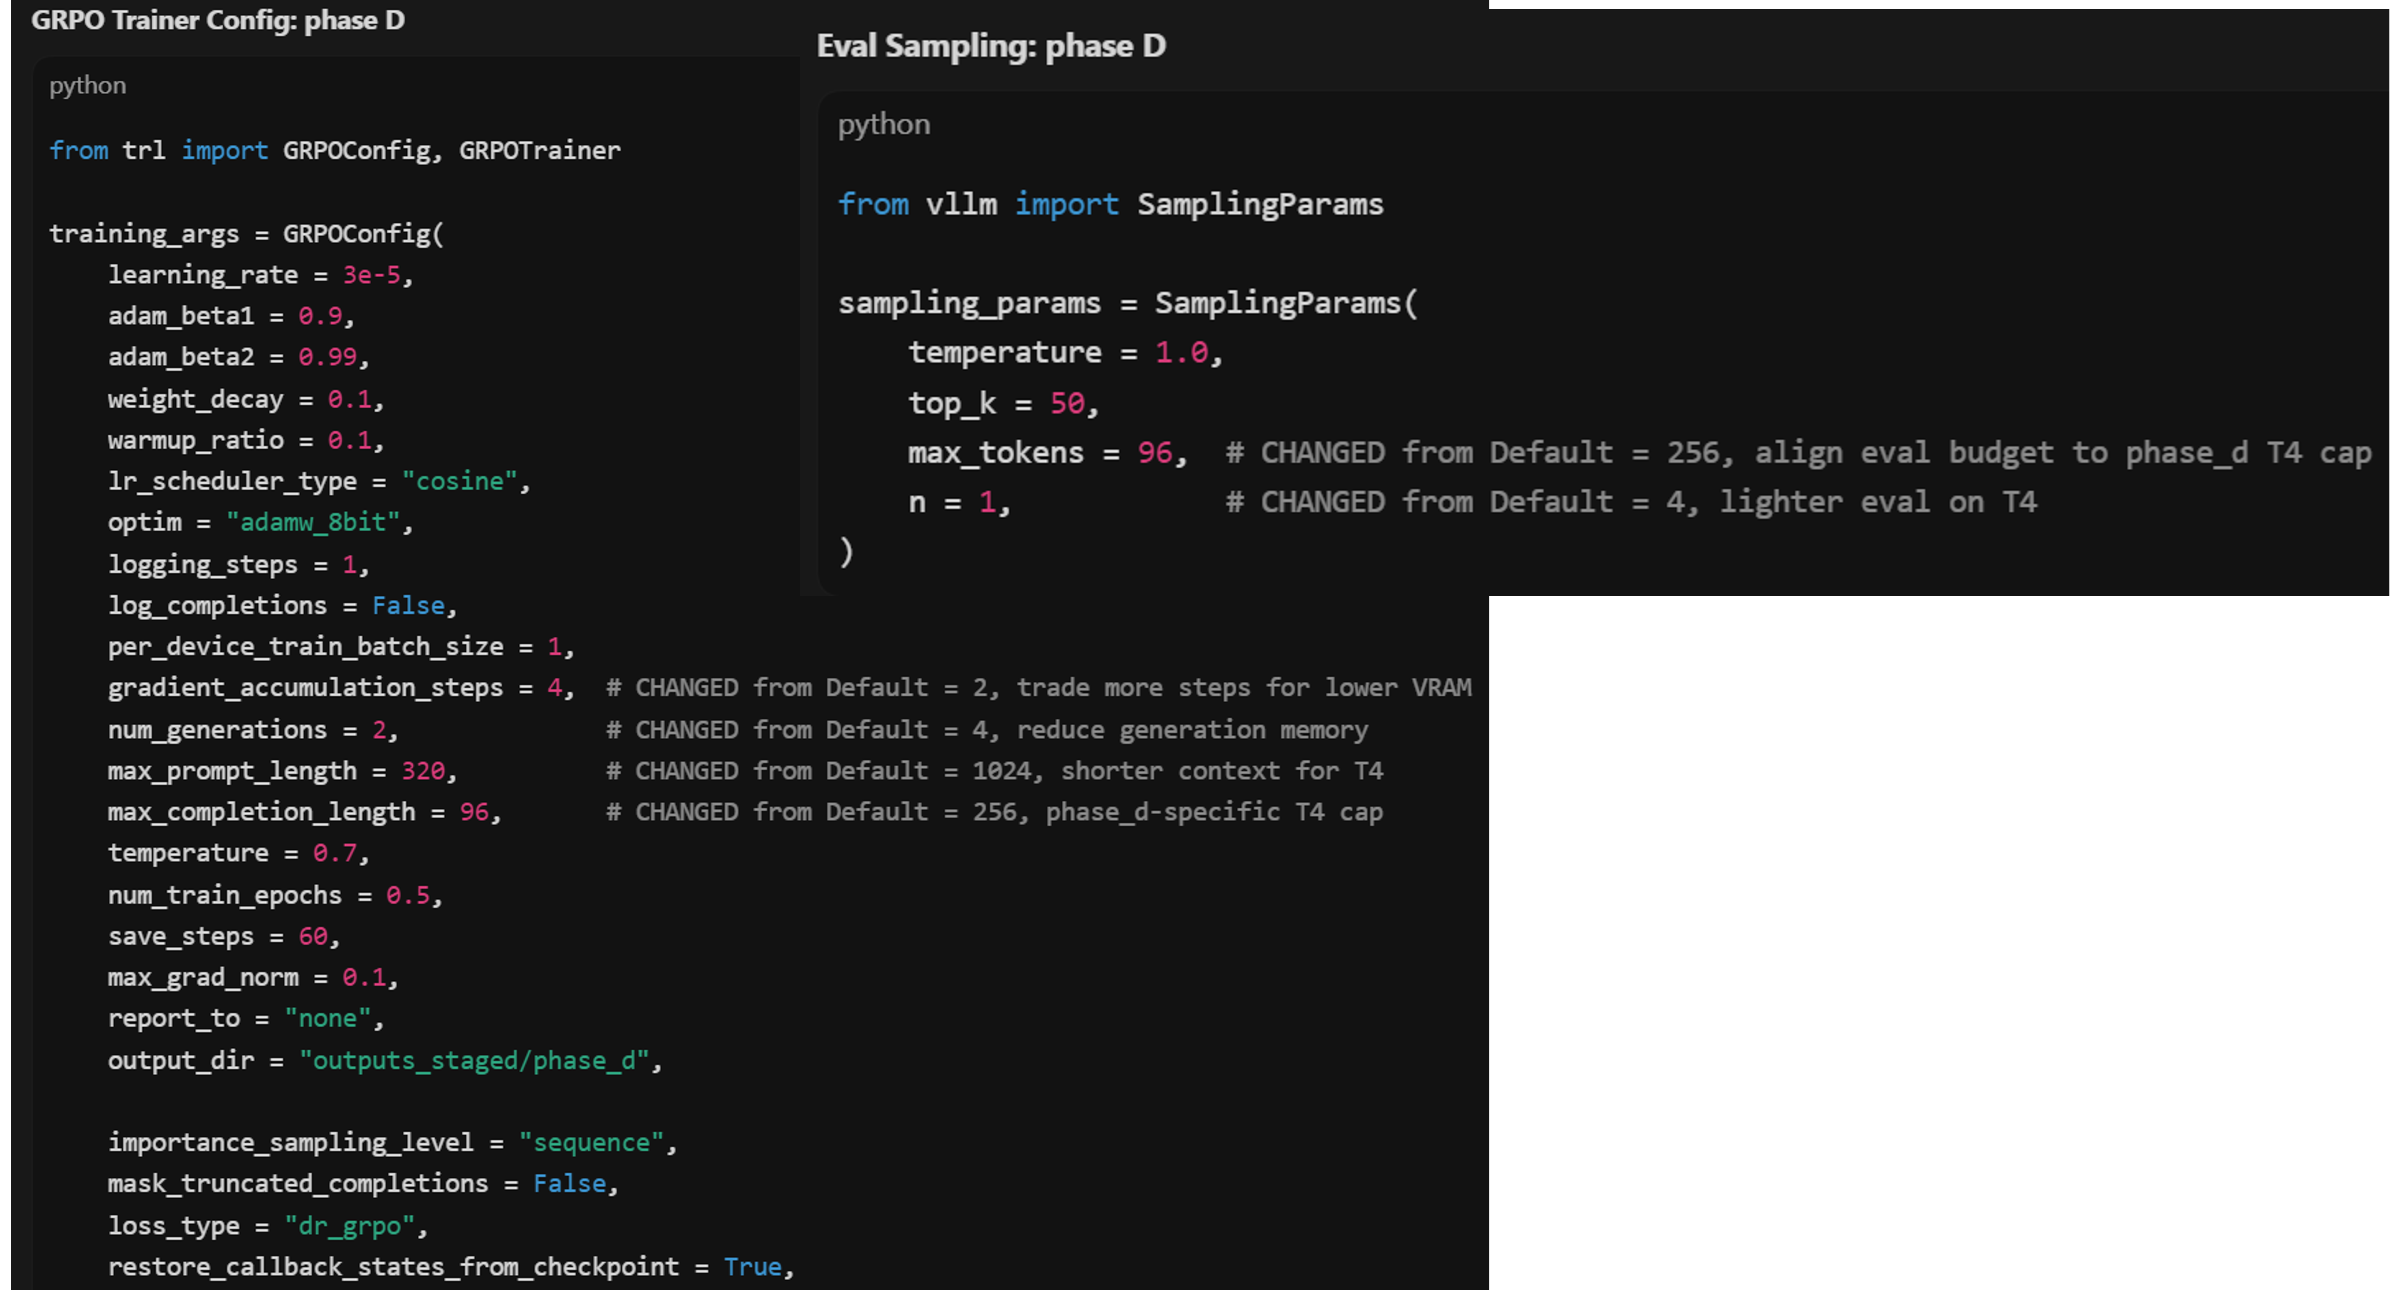
\includegraphics[width=\linewidth]{../../results/plots/Parameter_changes_2.png}
\caption{Additional parameter and phase-specific changes.}
\end{subfigure}
\caption{Supplementary implementation summaries for the low-memory training profile used by the successful runs. We keep these figures in the appendix because they support reproducibility more than they support the core algorithmic argument.}
\label{fig:param-changes}
\end{figure}

\end{document}
